\subsection{Сферическая тригонометрия}
\label{sec:spher-trig}
\begin{wrapfigure}[10]{r}{.3\tw}
	\centering
	\vspace{-1pc}
 	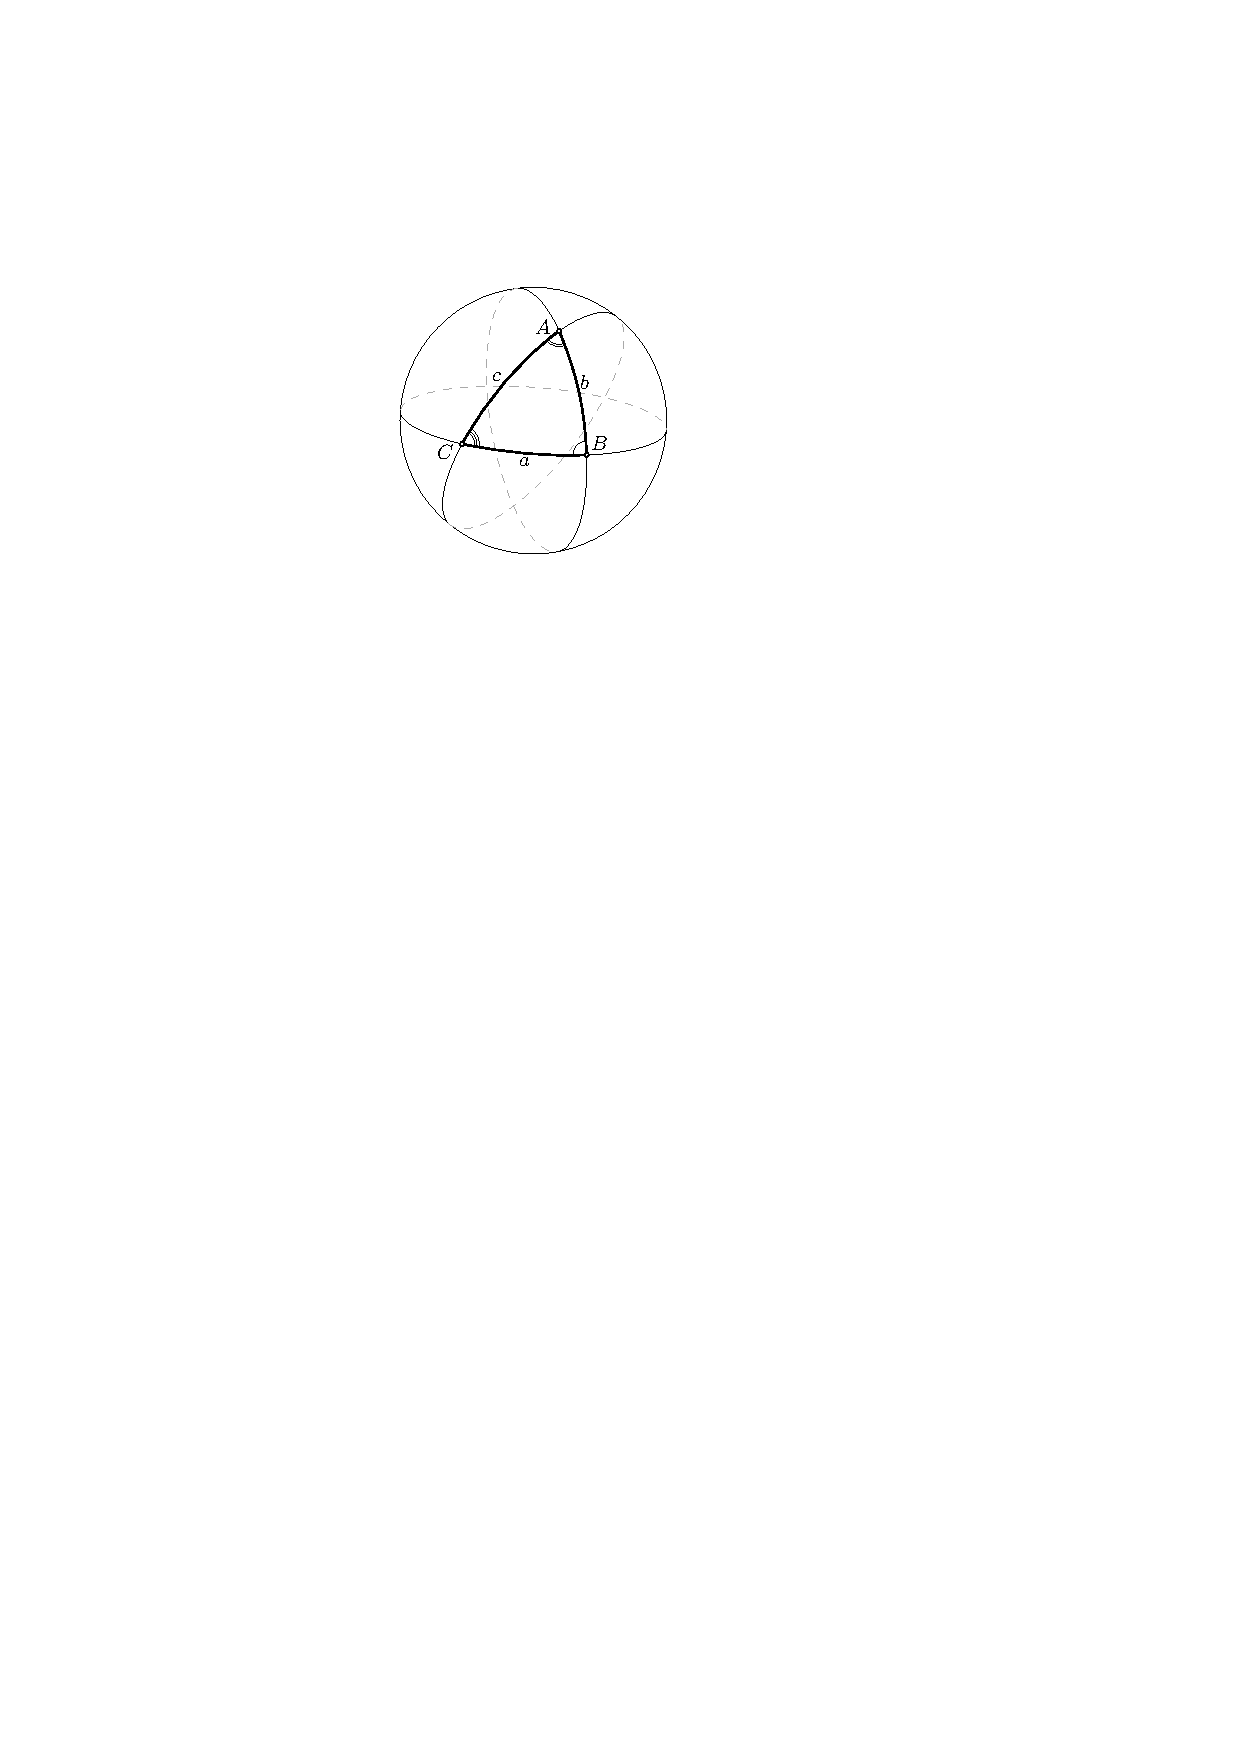
\includegraphics[width=0.3\textwidth]{spher-trigonom}
 	\caption{Сферический треугольник}
\end{wrapfigure}
Для решения некоторых задач астрономии, связанных с видимыми положениями небесных тел, требуются знания о сферической тригонометрии. \imp{Сферический треугольник}~--- фигура на поверхности сферы, состоящая из трёх точек и трёх дуг больших кругов, соединяющих эти точки. Пусть $A$, $B$ и $C$~--- углы сферического треугольника, а $a$, $b$ и $c$~--- его стороны.

Сферические треугольники обладают следующими свойствами:
\begin{enumerate}
\item Два сферических треугольника равны, если они подобны.
\item Каждая сторона меньше суммы двух других сторон и больше их разности.
\item Сумма всех сторон $a+b+c$ всегда меньше $2\pi$.
\item Сумма углов сферического треугольника $\pi < A + B + C < 3\pi$.
\item Разность суммы двух углов и третьего угла меньше $\pi$
\end{enumerate}

Площадь сферического треугольника определяется по формуле:
\begin{equation}
	S = R^2( A + B + C - \pi),
\end{equation}
где $A + B + C - \pi$~--- \imp{сферический избыток}.

Для сферического треугольника $ABC$ справедлива \term{сферическая теорема косинусов}, имеющая вид
\begin{equation}
\cos a=\cos b\cos c+\sin b\sin c\cos A.
\end{equation}
\term{Сферическая теорема синусов} для такого треугольника выглядит так:
\begin{equation}
\frac{\sin a}{\sin A} = \frac{\sin b}{\sin B} = \frac{\sin c}{\sin C}.
\end{equation}

\term{Параллактический треугольник}~--- треугольник на небесной  сфере, образованный пересечением небесного меридиана, вертикального круга и часового круга светила. \imp{Вертикальный круг}~--- большой круг небесной сферы, проходящий через надир, зенит и светило. \imp{Часовой круг}~--- большой круг небесной сферы, проходящий через полюса мира и наблюдаемое светило.

Применяя теоремы синусов и косинусов к параллактическому треугольнику, нетрудно получить следующие соотношения:
\begin{gather}
\cos z=\sin\varphi\sin\delta+\cos\varphi\cos\delta\cos t\\
\sin z\sin A=\cos\delta\sin t\\
\sin z\cos A=-\cos\varphi\sin\delta+\sin\varphi\cos\delta\cos t
\end{gather}